\documentclass[a4paper,11pt]{article}
\usepackage{mathtools}
\usepackage{amssymb}
\usepackage[cm]{fullpage}
\usepackage{fancyhdr}
\usepackage[ddmmyyyy]{datetime} 
\usepackage[]{graphicx}
\usepackage{hhline}
\usepackage{listings}
\usepackage{todonotes}
\usepackage{hyperref}
\usepackage{enumitem}
\usepackage{tcolorbox}
\usepackage{cleveref}

\graphicspath{{figures}}

% Settings for listings package
\definecolor{mygreen}{rgb}{0,0.6,0}
\definecolor{mygray}{rgb}{0.5,0.5,0.5}
\definecolor{mymauve}{rgb}{0.58,0,0.82}
\definecolor{altblue}{rgb}{0.0,0.6,1.0}
\definecolor{lstbg}{gray}{0.9}

\lstset{
  backgroundcolor=\color{lstbg},
  % choose the background color; you must add \usepackage{color} or \usepackage{xcolor}
  basicstyle=\footnotesize\ttfamily,
  % the size of the fonts that are used for the code
  breakatwhitespace=true,
  % sets if automatic breaks should only happen at whitespace
  breaklines=true,
  % sets automatic line breaking
  captionpos=b,
  % sets the caption-position to bottom
  commentstyle=\color{mygreen},
  % comment style
  deletekeywords={},
  % if you want to delete keywords from the given language
  escapeinside={\#*}{*},
  % if you want to add LaTeX within your code
  extendedchars=true,
  % lets you use non-ASCII characters; for 8-bits encodings only, does not work with UTF-8
  frame=single,
  % adds a frame around the code
  keepspaces=true,
  % keeps spaces in text, useful for keeping indentation of code (possibly needs columns=flexible)
  keywordstyle=\color{blue},
  % keyword style
  %language=c++,
  % the language of the code
  otherkeywords={},
  % if you want to add more keywords to the set
  numbers=left,
  % where to put the line-numbers; possible values are (none, left, right)
  numbersep=5pt,
  % how far the line-numbers are from the code
  numberstyle=\tiny\color{mygray},
  % the style that is used for the line-numbers
  rulecolor=\color{black},
  % if not set, the frame-color may be changed on line-breaks within not-black text (e.g. comments (green here))
  showspaces=false,
  % show spaces everywhere adding particular underscores; it overrides 'showstringspaces'
  showstringspaces=false,
  % underline spaces within strings only
  showtabs=false,
  % show tabs within strings adding particular underscores
  stepnumber=1,
  % the step between two line-numbers. If it's 1, each line will be numbered
  stringstyle=\color{mymauve},
  % string literal style
  tabsize=4,
  % sets default tabsize to 4 spaces
  title=\lstname
  % show the filename of files included with \lstinputlisting; also try caption instead of title
}

%[leftmargin=!,labelindent=0mm,labelwidth=0mm,labelsep=2mm,itemindent=0mm]
\newlist{boxlist}{itemize}{1}
\setlist[boxlist]{leftmargin=!,
					labelindent=0mm,
					labelwidth=0mm,
					%labelsep=2mm,
					itemindent=0mm}
\setlist[boxlist,1]{label=\textbullet}

\newenvironment{rbox}[1]{%
	\centering
	\tcolorbox[savedelimiter=rbox,
				width=2\linewidth/3,
				arc=3mm,
				boxrule=0.8mm,
				colframe=altblue!30,
				coltitle=black,
				colback=altblue!10,
				coltext=black,
				fonttitle=\large,
				title={#1}]}
	{\endtcolorbox}
	
\newenvironment{jacknotes}{\color{red}\renewcommand{\labelitemi}{$\star$}\begin{itemize}}{\end{itemize}}

\author{Jack Betteridge}

\pagestyle{fancy}
\setlength{\headheight}{15pt}
\setlength{\headsep}{5pt}
\lhead{ \fancyplain{}{} }
\rhead{ \fancyplain{}{} }
%\lhead[\footnotesize\nouppercase{\leftmark}]{}
%\rhead[]{\footnotesize\nouppercase{\rightmark}}

\renewcommand{\footrulewidth}{0.4pt}
\cfoot[-- \thepage\ --]{-- \thepage\ --}

% Macros
\newcommand{\RR}{\mathbb{R}}

\begin{document}
\begin{center}
\textsc{\Large Firedrake}\\
\textsc{2021 Code Performance Series: From analysis to insight}
\end{center}

Attended by:
\begin{itemize}
	\item Jack Betteridge
	\item Josca Fregin
	\item Reuben Nixon-Hill
	\item Sophia Vorderwuelbecke
	\item Connor Ward
\end{itemize}

%%%%%%%%%%%%%%%%%%%%%%%%%%%%%%
\section{Overview}
\label{sec:overview}
%%%%%%%%%%%%%%%%%%%%%%%%%%%%%%
\begin{jacknotes}
	\item Summarise what Firedrake is and how it works
\end{jacknotes}
\begin{quote}
\emph{``Firedrake is an automated system for the solution of partial differential equations using the finite element method (FEM). Firedrake uses sophisticated code generation to provide mathematicians, scientists, and engineers with a very high productivity way to create sophisticated high performance simulations.''}
\end{quote}


%%%%%%%%%%%%%%%%%%%%%%%%%%%%%%
\section{Case Study}
\label{sec:case}
%%%%%%%%%%%%%%%%%%%%%%%%%%%%%%
\subsection{Mathematical Problem}
\label{ssec:maths}
%%%%%%%%%%%%%%%%%%%%%%%%%%%%%%
We consider Poisson's equation in a 3D domain $\Omega=[0,1]^3\subset\RR^3$ with homogeneous Dirichlet boundary conditions:
\begin{equation}
\left\{
\begin{aligned}
	-\nabla^2 u &= f && \text{on } \Omega\\
	u &= 0 && \text{on } \partial\Omega
\end{aligned}
\right.
\end{equation}
With a manufactured solution
\begin{equation}
	u(x, y, z) = \sin(\pi x)\tan\left(\frac{\pi x}{4}\right)\sin(a\pi y)\sin(b\pi z)
\end{equation}
corresponding to a right-hand side
\begin{equation}
	f(x, y, z) = \frac{\pi^2}{2}
	%\left( 2(a^2 + b^2)\cos(\pi x) - (4a^2 + b^2 + 1)\cos \left( \frac{\pi x}{2}\right) + 2(a^2 + b^2) \right) 
	\left( 2\cos(\pi x) - \cos\left( \frac{\pi x}{2} \right) - 2(a^2 + b^2)\sin(\pi x)\tan \left( \frac{\pi x}{4} \right)  \right) 
	\sin(a\pi y) \sin(b\pi z).
\end{equation}
For these experiments we fix $a=1$ and $b=2$.

%%%%%%%%%%%%%%%%%%%%%%%%%%%%%%
\subsection{Code}
\label{ssec:code}
%%%%%%%%%%%%%%%%%%%%%%%%%%%%%%
\begin{lstlisting}
poisson_gmg.py [-h] [--baseN BASEN] [--nref NREF] [--degree DEGREE]
                      [--resultsdir RESULTSDIR]
                      [--solver_params {LU,LU MUMPS,LU SuperLU_dist,MG V-cycle,MG F-cycle,MG F-cycle matfree,MG F-cycle LU coarse MUMPS,MG F-cycle LU coarse SuperLU_dist,MG F-cycle Cholesky coarse MUMPS,MG F-cycle Cholesky coarse SuperLU_dist,MG F-cycle PatchPC,MG F-cycle PatchPC telescope,MG F-cycle PatchPC telescope SuperLU_dist,MG F-cycle ASMStarPC,MG F-cycle ASMStarPC TinyASM}]
                      [--telescope_factor TELESCOPE_FACTOR]

optional arguments:
  -h, --help            show this help message and exit
  --baseN BASEN         base mesh size
  --nref NREF           number of mesh refinements
  --degree DEGREE       degree of CG element
  --resultsdir RESULTSDIR
                        directory to save results in
  --solver_params {LU,LU MUMPS,LU SuperLU_dist,MG V-cycle,MG F-cycle,MG F-cycle matfree,MG F-cycle LU coarse MUMPS,MG F-cycle LU coarse SuperLU_dist,MG F-cycle Cholesky coarse MUMPS,MG F-cycle Cholesky coarse SuperLU_dist,MG F-cycle PatchPC,MG F-cycle PatchPC telescope,MG F-cycle PatchPC telescope SuperLU_dist,MG F-cycle ASMStarPC,MG F-cycle ASMStarPC TinyASM}
                        name of dict to take solver parameters from
  --telescope_factor TELESCOPE_FACTOR
                        Telescope factor for telescoping solvers (set to number of NODES)

\end{lstlisting}

\verb`baseN` corresponds to the size of the coarsest grid in the multigrid solver and \verb`nref` corresponds to the number of multigrid levels minus 1.

Example usage:

\begin{lstlisting}
mpiexec -n 8 python poisson_gmg.py \
    --resultsdir results/poisson_patch \
    --baseN 12 \
    --nref 3 \
    --solver_params "MG F-cycle PatchPC" \
    --telescope_factor 1
\end{lstlisting}

\subsubsection*{Different solvers:}
Direct solvers:
\begin{itemize}
	\item LU: Direct solver using PETSc built in LU factorisation.
    \item LU MUMPS: Direct solver using MUMPS LU factorisation.
	\item LU SuperLU\_dist: Direct solver using SuperLU\_dist LU factorisation.
\end{itemize}

\noindent(Geometric) Multigrid solvers:
\begin{itemize}
	\item MG V-cycle: A conjugate gradient (CG) Krylov Subspace solver (KSP) with multigrid (MG) V-cycle preconditioner (PC).
    \item MG F-cycle: Full MG preconditioner (no KSP).
    \item MG F-cycle matfree: Full MG PC using firedrake.AssembledPC and telescoping (and SuperLU\_dist LU factorisation on coarsest grid).
    \item MG F-cycle LU coarse MUMPS: Full MG PC with direct solver using MUMPS LU factorisation on coarsest grid.
    \item MG F-cycle LU coarse SuperLU\_dist: Full MG PC with direct solver using SuperLU\_dist LU factorisation on coarsest grid.
    \item MG F-cycle Cholesky coarse MUMPS: Full MG PC with direct solver using MUMPS Cholesky factorisation on coarsest grid.
    \item MG F-cycle Cholesky coarse SuperLU\_dist: Full MG PC with direct solver using MUMPS Cholesky factorisation on coarsest grid.
\end{itemize}

\noindent(Geometric) Multigrid with PatchPC:
\begin{itemize}
	\item MG F-cycle PatchPC: Full MG PC using firedrake.PatchPC to apply star smoothing (and MUMPS LU factorisation on coarsest grid).
    \item MG F-cycle PatchPC telescope: Full MG PC using firedrake.PatchPC to apply star smoothing, with telescoping (and MUMPS LU factorisation on coarsest grid).
    \item MG F-cycle PatchPC telescope SuperLU\_dist: Full MG PC using firedrake.PatchPC to apply star smoothing, with telescoping and SuperLU\_dist LU factorisation on coarsest grid.
    \item MG F-cycle ASMStarPC: Full MG PC using firedrake.ASMStarPC to apply star smoothing (and MUMPS LU factorisation on coarsest grid).
    \item MG F-cycle ASMStarPC TinyASM: Full MG PC using firedrake.ASMStarPC and the TinyASM backend to apply star smoothing (and MUMPS LU factorisation on coarsest grid).
\end{itemize}
    


%%%%%%%%%%%%%%%%%%%%%%%%%%%%%%
\section{Current methodology}
\label{sec:current}
%%%%%%%%%%%%%%%%%%%%%%%%%%%%%%
Using multiple languages, there are various different profiling tools and techniques used by developers and users of the Firedrake project.

The most straightforward utilised Python's own built in profiling tools.
Simply invoking any Firedrake script with the cProfile tool generates a profile that can be read in with the \verb`pstats` library.
Alternatively an interactive flamegraph can be generated in a web browser using a tool like \verb`snakeviz`.
\begin{lstlisting}[language=bash]
	python -m cProfile my_firedrake_script.py
	mpiexec -n 1 python -m cProfile my_firedrake_script.py : -n 7 python my_firedrake_script.py
\end{lstlisting}

Statistical Python profilers can also be used like \verb`pyinstrument` or \verb`pyspy` can be used as a less invasive alternative.
\verb`pyspy` in particular is very useful as it allows not only the statistical profiling of Python calls, but also C kernels that Firedrake calls out too.

PETSc is used extensively within Firedrake, by utilising the PETSc data structures for meshes, vectors and matrices it allows for the use of the extensive library of linear and non-linear solvers.
For this reason, PETSc's internal instrumentation is often used for profiling and tracing.
\begin{lstlisting}[language=bash]
	mpiexec -n 8 python my_firedrake_script.py -log_view
	mpiexec -n 8 python my_firedrake_script.py -log_view:log.py:ascii_info_detail
	mpiexec -n 8 python my_firedrake_script.py -log_view:log.xml:ascii_xml
	mpiexec -n 8 python my_firedrake_script.py -log_all
	mpiexec -n 8 python my_firedrake_script.py -log_trace
\end{lstlisting}
Often it is sufficient to display a summary of the profile to stdout, which is what the \verb`-log_view` command line argument provides.
This textual summary can be saved to a text file, or written to a Python script or XML document for later processing.

Through \verb`petsc4py`, \verb`pyop2` provides utilities to add timed functions and timed regions to users code, which will appear in the resultant log view.

In response for the need for more end user profiling, two additional utilities have been developed to help process the profiles generated by PETSc.
The first \verb`petsc-xml2flamegraph`, developed by Connor Ward takes the XML formatted output from PETSc log view and puts it into a standard format for generating a flamegraph.
\Cref{fig:flame} shows an example of one such flame graph based on a run of our example problem on 256 cores of DINE.
\begin{figure}[htp]
	\centering
	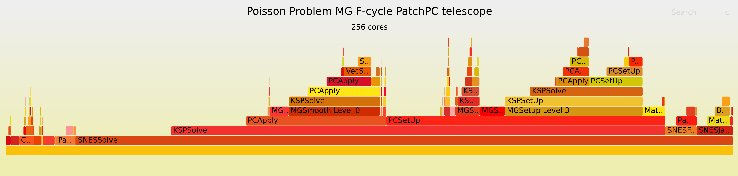
\includegraphics[width=\textwidth]{256_flame.pdf}
	\label{fig:flame}
	\caption{Flame graph}
\end{figure}
This tool is discussed in greater detail in \cref{ssec:scorep}.
The second developed by Jack Betteridge takes several Python formatted output files from PETSc log view, which form part of a scaling experiment and plot the scaling of selected components.
\Cref{fig:component} shows an example of the scaling of the PETSc KSP solver over a strong scaling run on the DINE cluster, from 32 cores (1 node) to 256 (8 nodes).
\begin{figure}[htp]
	\centering
	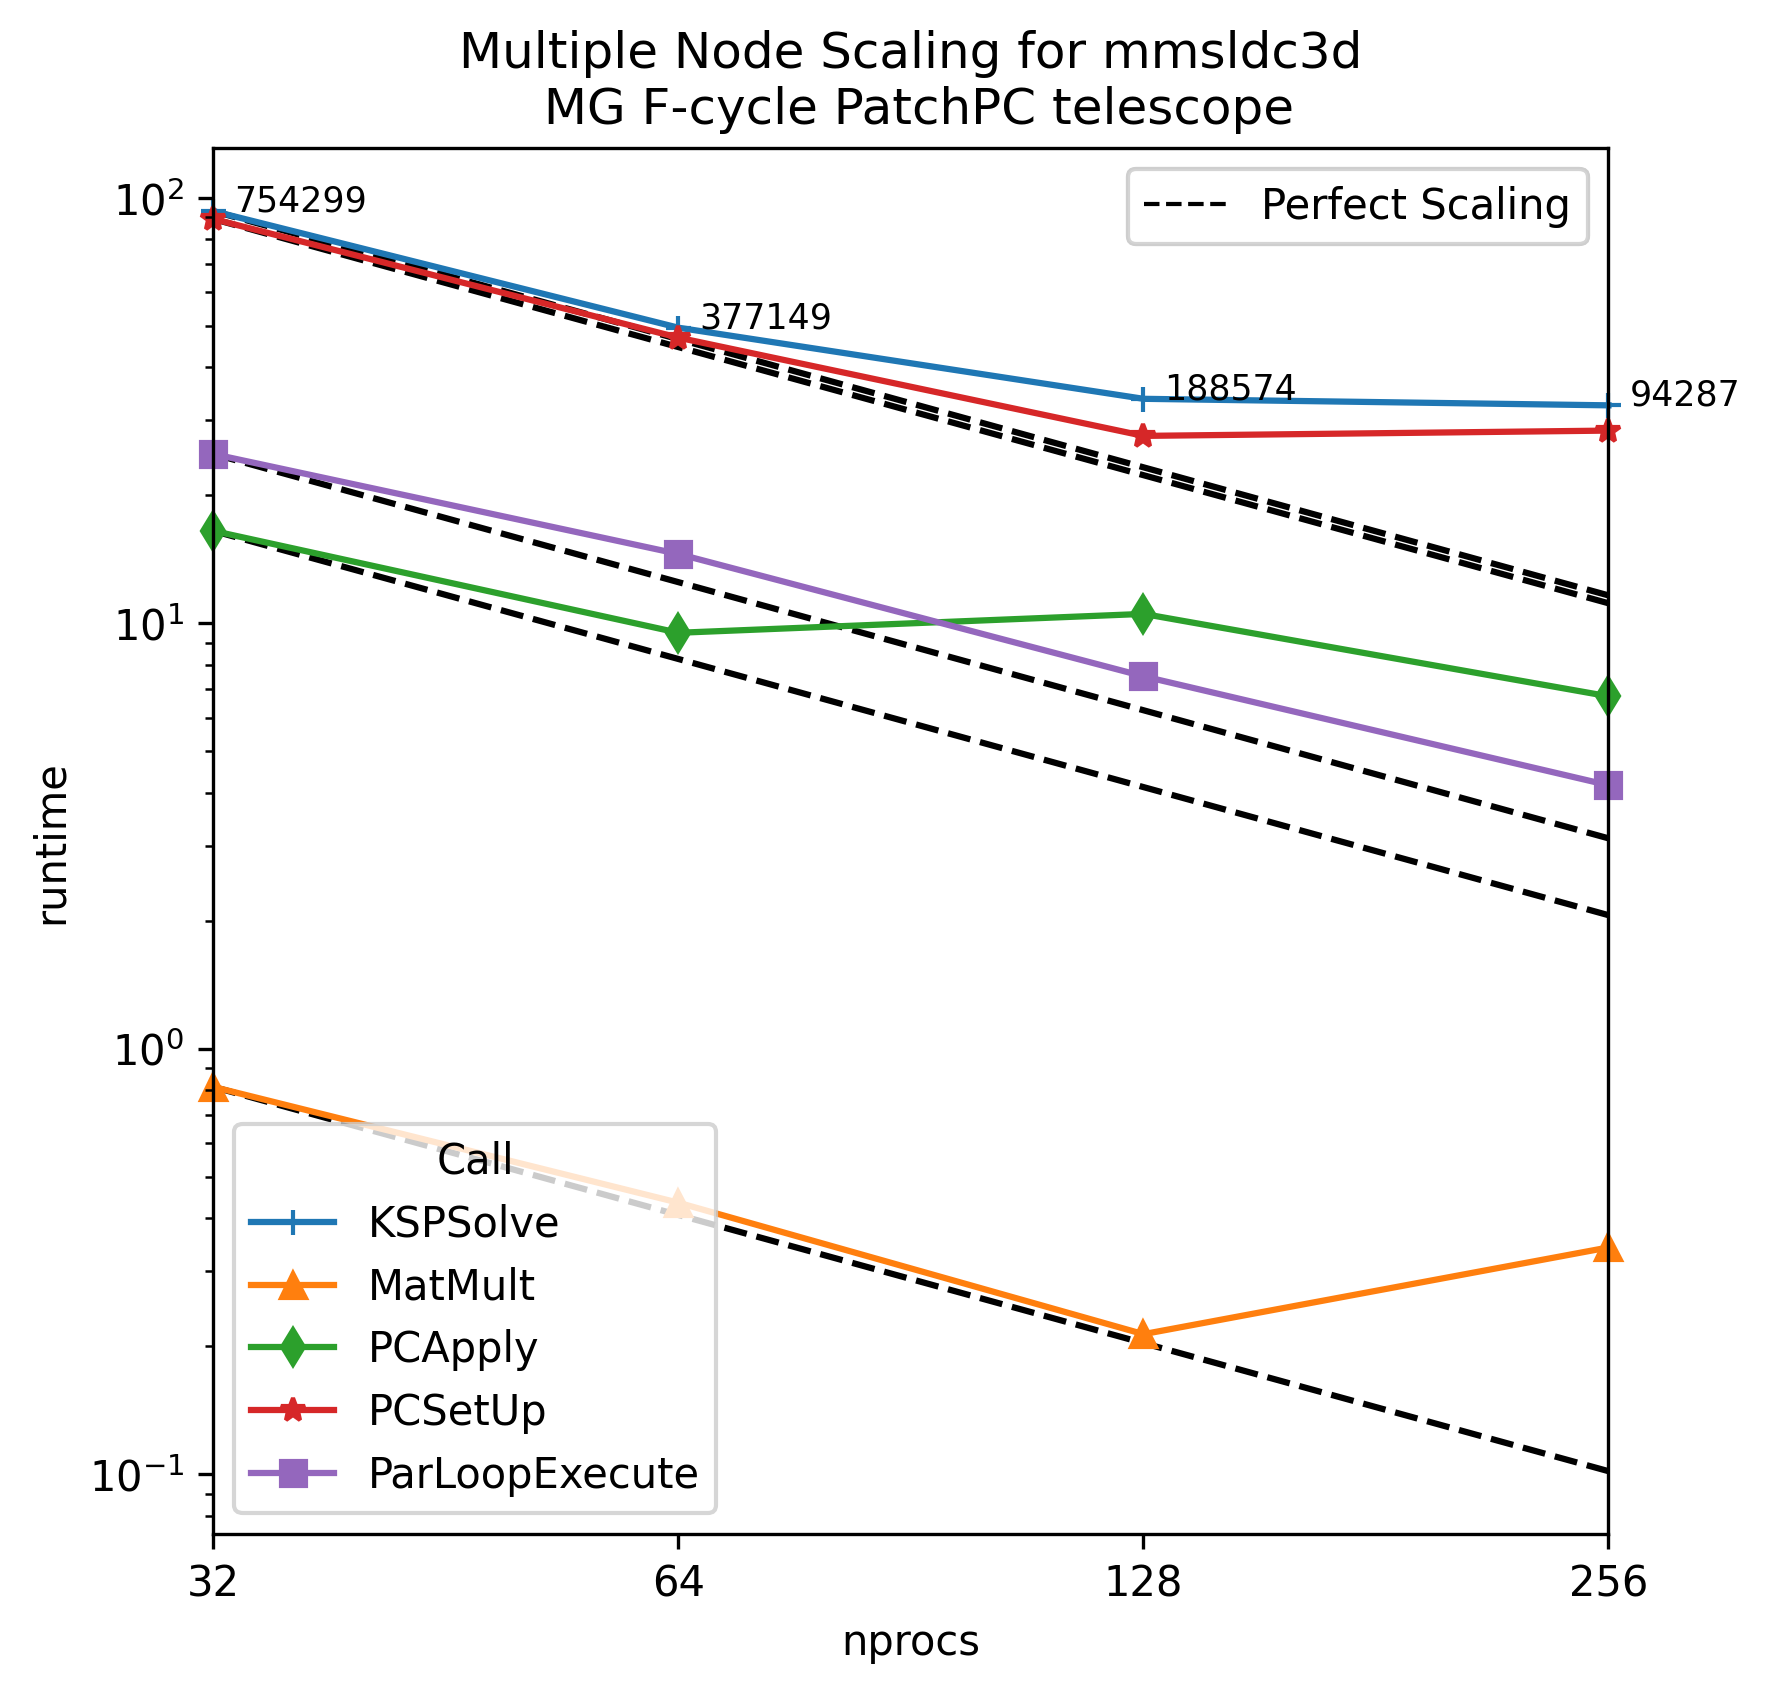
\includegraphics[width=0.5\textwidth]{main_stage_absolute.png}
	\label{fig:component}
	\caption{Component scaling}
\end{figure}


%%%%%%%%%%%%%%%%%%%%%%%%%%%%%%
\section{Aims}
\label{sec:aims}
%%%%%%%%%%%%%%%%%%%%%%%%%%%%%%
\begin{jacknotes}
	\item Scaling and performance of PyOP2 (Connor)
	\item Scaling and performance of different solvers within PETSc (Jack)
	\item Vectorisation experiments? (Sophia?)
\end{jacknotes}


\clearpage
%%%%%%%%%%%%%%%%%%%%%%%%%%%%%%
\section{Session diary}
\label{sec:diary}
%%%%%%%%%%%%%%%%%%%%%%%%%%%%%%
\subsection*{21/01/2021 - ARM and Intel performance tools}
\label{ssec:arm_intel}
%%%%%%%%%%%%%%%%%%%%%%%%%%%%%%
\begin{jacknotes}
	\item Preparations JB: installing Firedrake
	\item Discuss Intel tool (and it not working \textbf{at all})
	\item Allinear DDT not working at time
\end{jacknotes}
\subsubsection*{Preparations}
The most essential step in our preparations for the first workshop was getting Firedrake installed and tested on the DINE cluster.

\subsubsection*{Session}
The session focussed on using the two commercial tools:
\begin{enumerate}
	\item \verb`aps` (Application Performance Spnapshot) part of Intel Vtune
	\item \verb`perftool` part of ARM Forge (which includes ARM DDT, formerly Allinear DDT)
\end{enumerate}

We briefly document the Intel tool here as a record of what was run, but we never actually got anyperformance information out of \verb`aps`.
\begin{lstlisting}
mpiexec -np n [...] \
	aps -r aps_myprog --collection-mode=mpi \
		./myprog [args]
\end{lstlisting}

The ARM tool was a bit more promising, we managed to produce a serial performance result during the session.
\begin{lstlisting}
perf-report \
	mpiexec -np n [...] \
		./myprog [args]
\end{lstlisting}

\subsubsection*{Follow up}
After installing our own Python and rebuilding Firedrake to use the system OpenMPI 4.0.5, we used \verb`perftool` to generate performance reports for some parallel experiments.
We had no such luck with Intel.

Take aways
\begin{itemize}
	\item These profiling tools are primarily designed for monolithic codes, where recompiling with different tools is a straightforward process.
\end{itemize}

\clearpage
%%%%%%%%%%%%%%%%%%%%%%%%%%%%%%
\subsection{18/02/2021 - ScoreP}
\label{ssec:scorep}
%%%%%%%%%%%%%%%%%%%%%%%%%%%%%%
\begin{jacknotes}
	\item Preparations JB: installing Python CW: Installing PETSc
	\item Discuss bug
	\item Discuss Connor's new tool
\end{jacknotes}
\subsubsection*{Preparations}
We built our own Python distribution to use with Firedrake as this was causing issues with the commercial tools, and building from scratch gave us more control over the toolchain.
For instance we knew our python was built with the GCC compilers version 10.2.1, the same as the system OpenMPI 4.0.5 with instrumentation and profiling support.
We were given fair warning that to do any profiling in the workshop on 18th February, our code should work with GCC 10.2.1 and OpenMPI 4.0.5 or the latest Intel tools available on DINE.


\subsubsection*{Session}
It quickly became apparent during the session that we were hitting issues profiling our code and what followed was essentially a debugging session, which we briefly outline.

During this time Connor Ward took the opportunity to introduce the rest of the team to the \verb`petsc-xml2flamegraph` tool, and how that could be used to profile a Firedrake script.

\subsubsection*{Follow up}
In response to the dubugging during the session, we went away and built the nightly release of ScoreP to verify whether the bug found was still present.
It wasn't, and we were able to start profiling our code.

\clearpage
%%%%%%%%%%%%%%%%%%%%%%%%%%%%%%
\subsection{11/03/2021 - Vampir}
\label{ssec:vampir}
%%%%%%%%%%%%%%%%%%%%%%%%%%%%%%
\begin{jacknotes}
	\item Preparations JB: installing ScoreP
\end{jacknotes}
\subsubsection*{Preparations}

\subsubsection*{Session}

\subsubsection*{Follow up}

\clearpage
%%%%%%%%%%%%%%%%%%%%%%%%%%%%%%
\section{Selected Results}
\label{sec:results}
%%%%%%%%%%%%%%%%%%%%%%%%%%%%%%


\clearpage
%%%%%%%%%%%%%%%%%%%%%%%%%%%%%%
\section{Conclusions and Future work}
\label{sec:conc}
%%%%%%%%%%%%%%%%%%%%%%%%%%%%%%

\begin{itemize}
	\item 
\end{itemize}

\clearpage
\section*{Acknowledgements}
The Firedrake team would like to thank:
\begin{description}
	\item[Tobias Weinzierl] for accepting our application to take part in the workshop series and organising the workshops.
	\item[Alastair Basden] for his assistance initially getting set up on DINE, and his help with queries throughout.
	\item[Brian Wylie] for his assistance, especially throughout the first session using the commercial tools and helping diagnose issues with our initial install.
	\item[Bill Williams] for his assistance, especially throughout the second session helping to debug and track down an issue in the system install of ScoreP.
\end{description}

This work has used Durham University's DINE cluster. DINE has been purchased through Durham University’s Research Capital Equipment Fund 19\_20 Allocation, led by the Department of Computer Science. It is installed in collaboration and as addendum to DiRAC\@Durham facility managed by the Institute for Computational Cosmology on behalf of the STFC DiRAC HPC Facility (\url{www.dirac.ac.uk}). DiRAC equipment was funded by BEIS capital funding via STFC capital grants ST/P002293/1, ST/R002371/1 and ST/S002502/1, Durham University and STFC operations grant ST/R000832/1. DiRAC is part of the National e-Infrastructure.

\end{document}
